\documentclass[12pt]{article}

%%%%% Preamble

%% Packages to use

\usepackage{amsmath,amsfonts,amssymb}   %% AMS mathematics macros
\usepackage{graphicx} %% Package to import images.
\usepackage{pagecolor}% http://ctan.org/pkg/{pagecolor}
\usepackage{float}



%% Title Information.
\title{The Unit's Resources v0.2.0}
\author{Ibai Basabe}
\date{}           %% By default, LaTeX uses the current date

%%%%% The Document

\begin{document}


\pagecolor{white}

\maketitle

\begin{abstract}

The Unit is the community-managed crypto-native unit of account for the metaverse. Here we describe The Unit governance resources in details.

\end{abstract}

\tableofcontents
\newpage



\section{Introduction}

In this document, we describe the distribution of The Unit resources. The Unit governance is the DAO that governs The Unit's main algorithm and processes to establish an index that can serve as a crypto benchmark and a crypto-native unit of account. For a complete description of The Unit main algorithm, see \cite{B1}.

\subsection{Note about the Usage of this Document}

This document has been prepared for information purposes only. It is not soliciting any action from the reader. The contents of this document are subject to change.


\section{Resource Economics}

\subsection{The Unit's Resources}

The Unit governance token is the controlling voting unit governing The Unit algorithm. The maximum amount to ever enter circulation is $2^{33}$ The Unit governance tokens.





\newpage

\subsection{Allocation}

We allocate The Unit's resources as shown in Figure \ref{fig:allocation}. 

\begin{figure}[h!]
\centering
  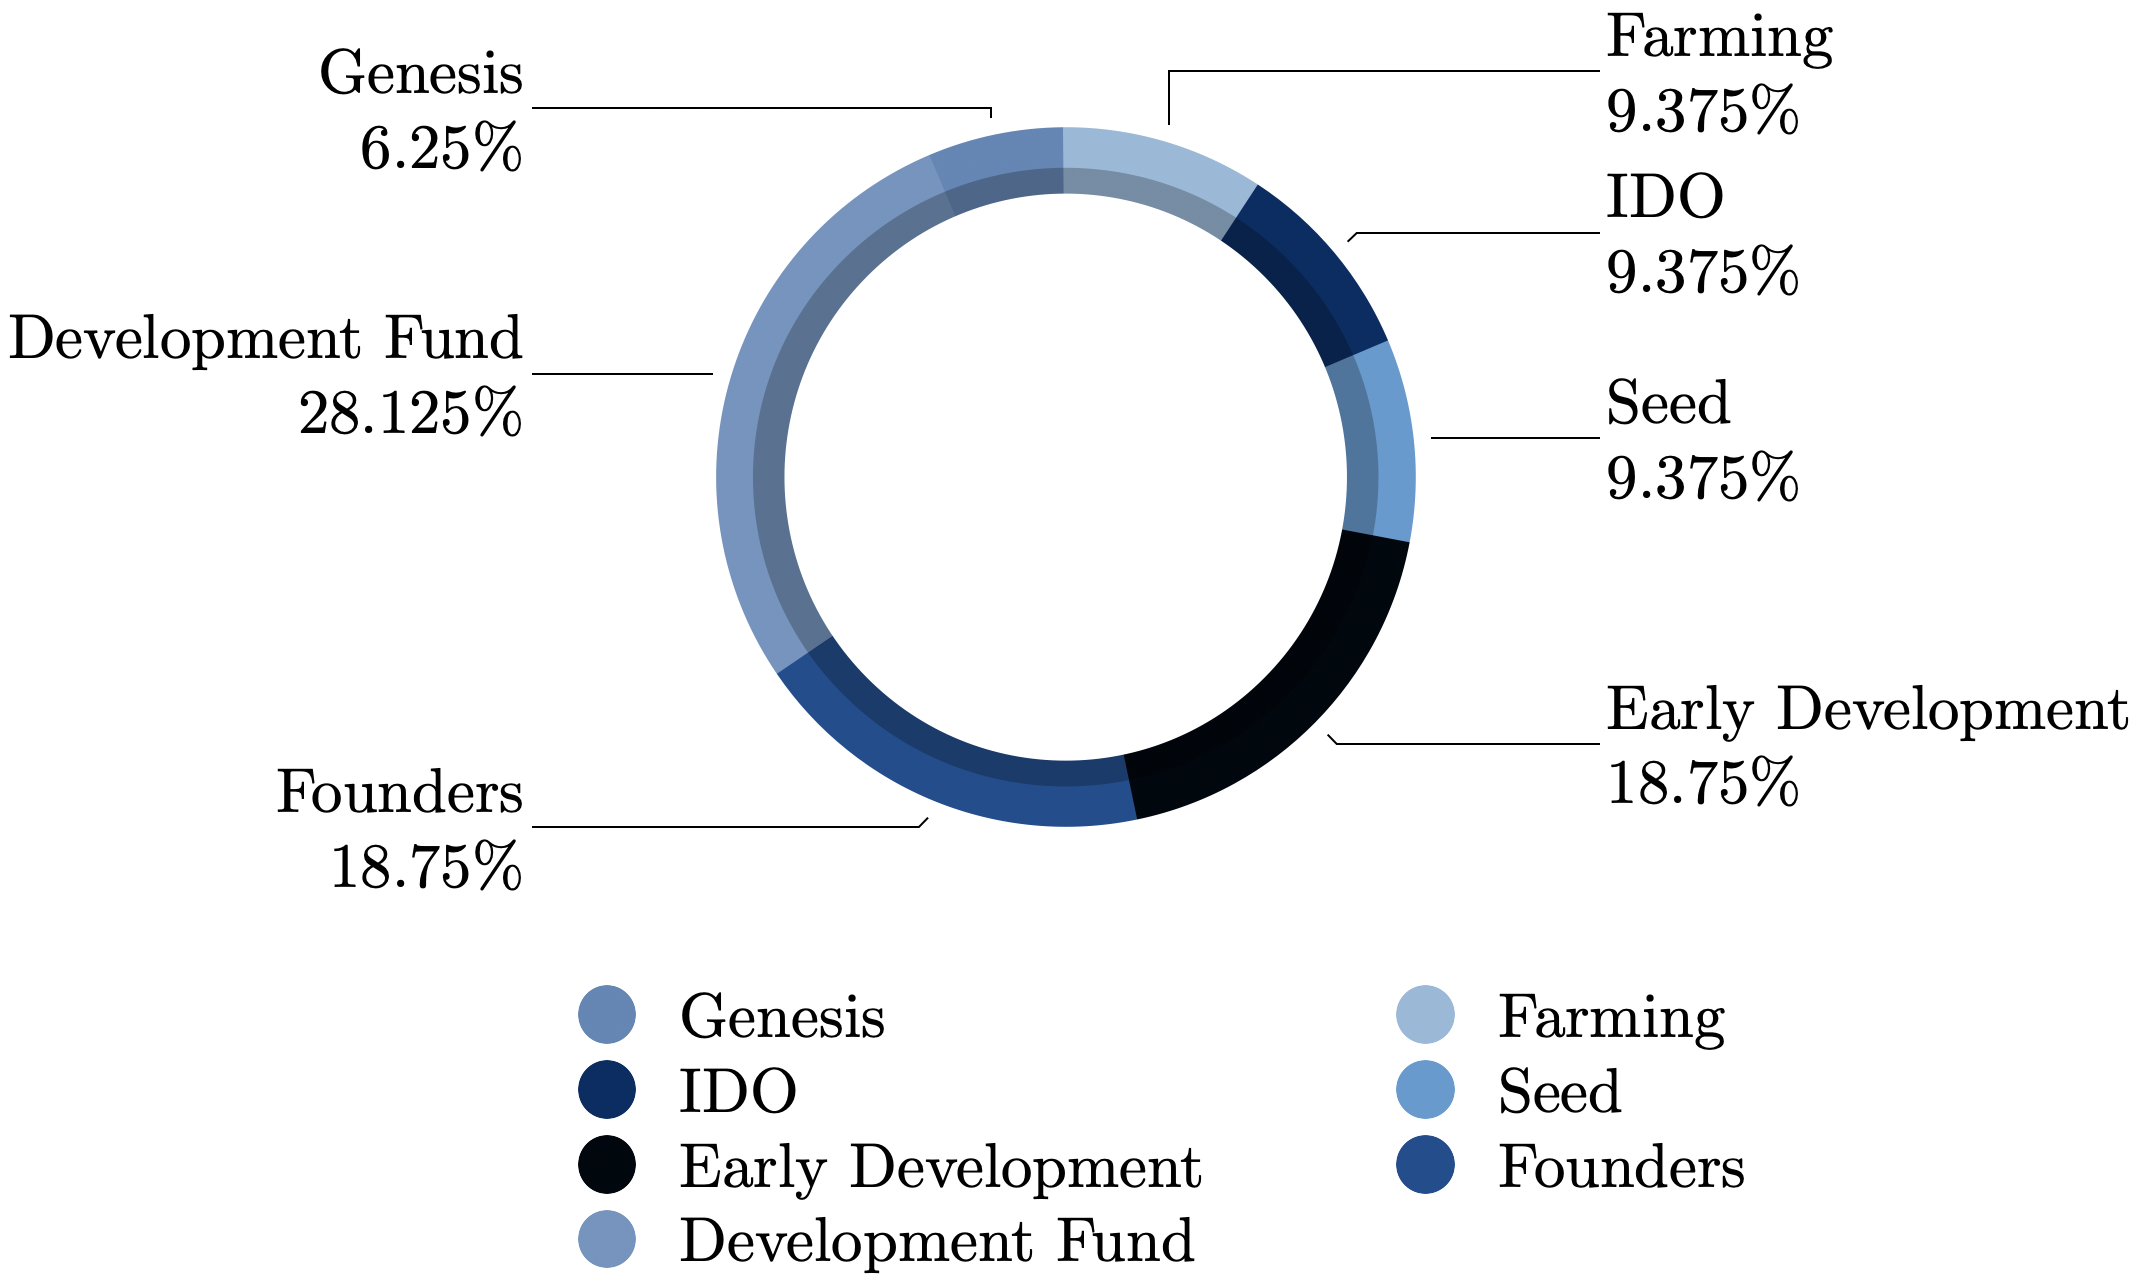
\includegraphics[width=5in]{images/The_Unit_Allocation.png}
  \caption{Total allocation.}
  \label{fig:allocation}
\end{figure}



\subsection{Vesting}

An amount of the initial The Unit's resources will be vested for the times defined in Figure \ref{fig:allocation_table}. Founders, Early Development, Seed, and Development Fund will have vesting schedules. For an allocation schedule with inflation rates see Figure \ref{fig:allocation_table2}.


\begin{figure}[H]
\centering
  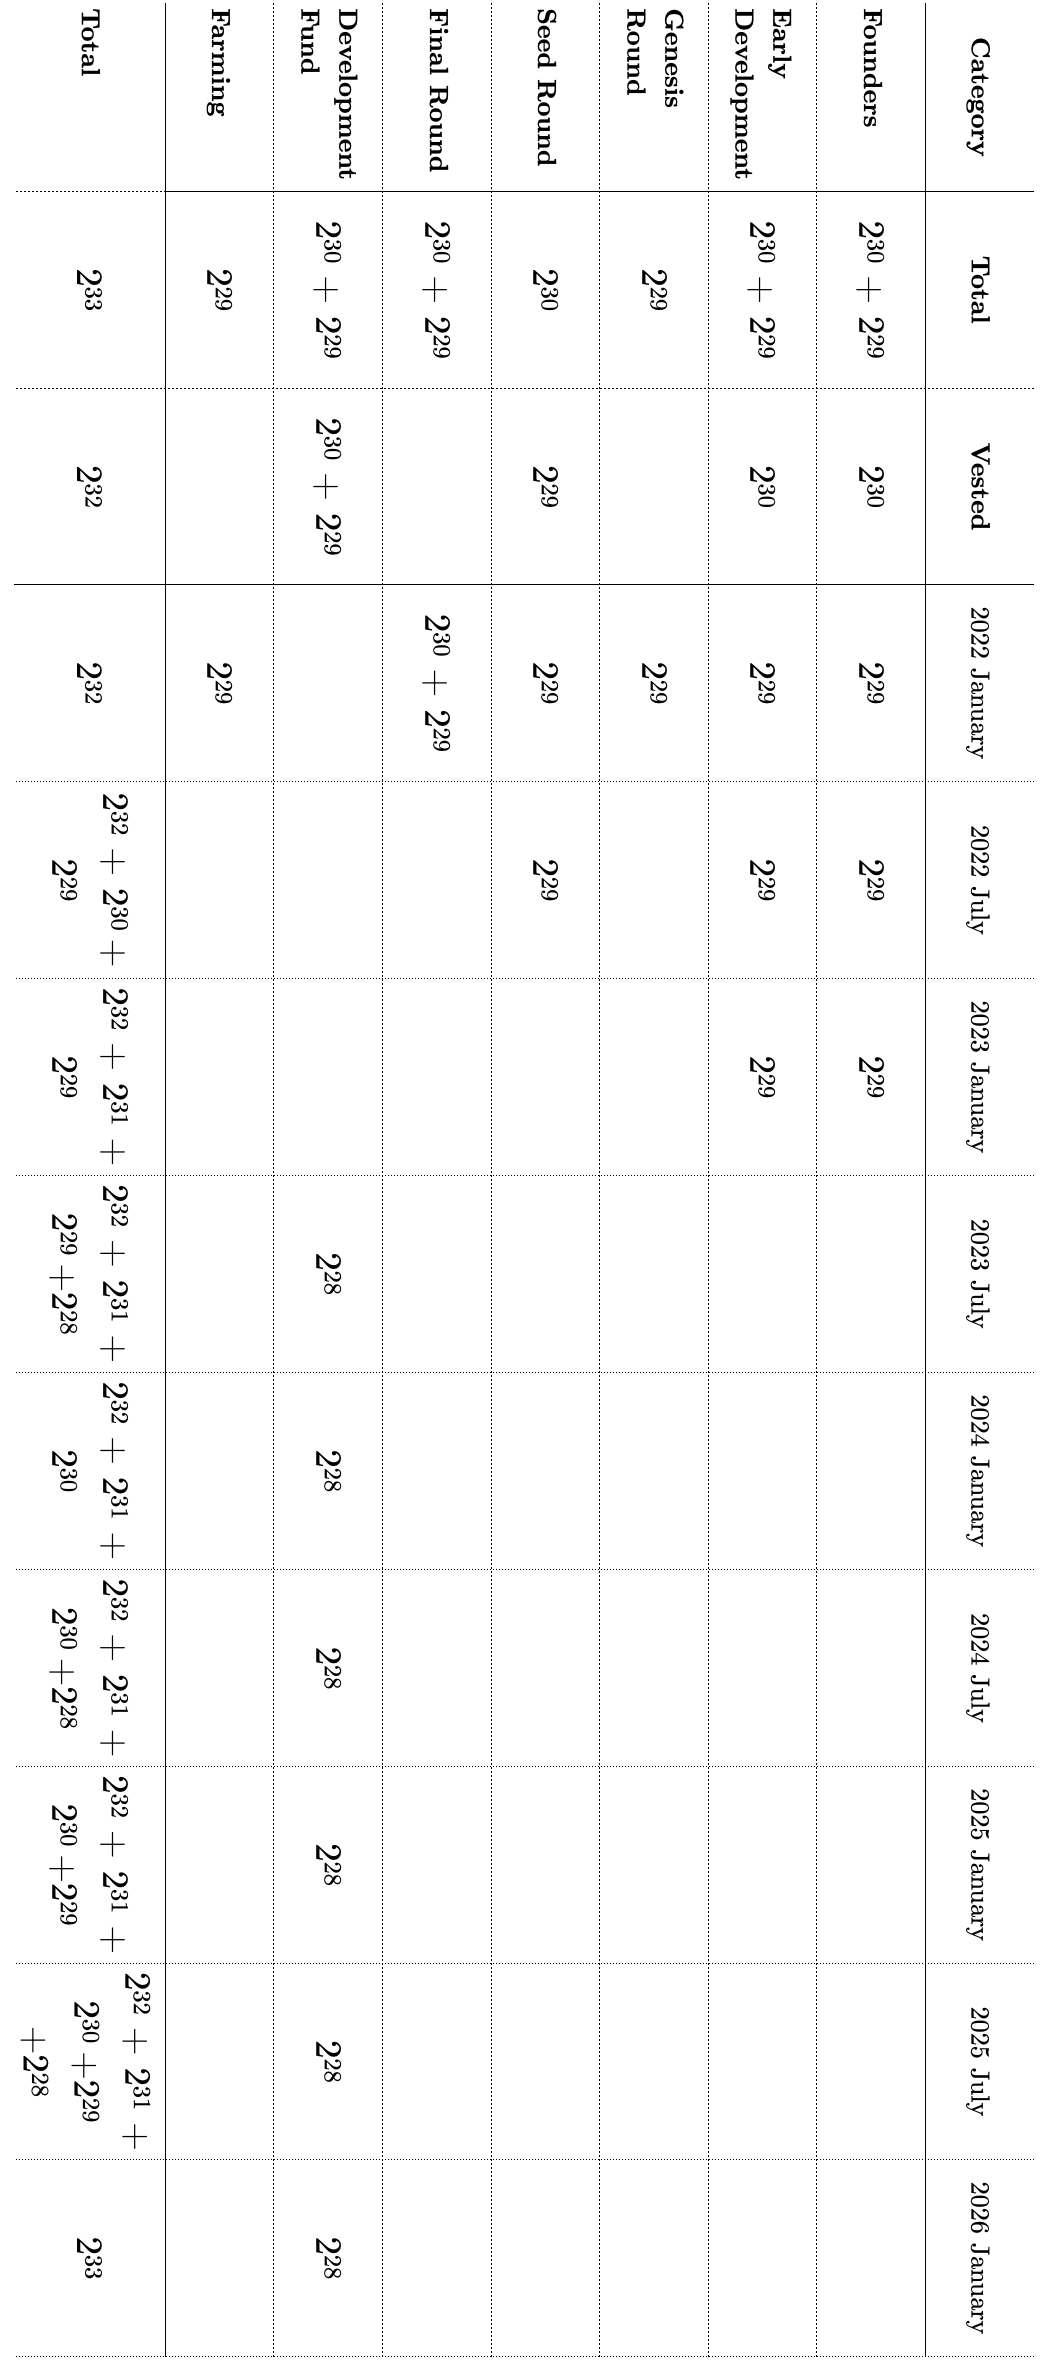
\includegraphics[width=3.5in]{images/The_Unit_Allocation_Table.png}
  \caption{Allocation with vesting details}
  \label{fig:allocation_table}
\end{figure}



\begin{figure}[H]
\centering
  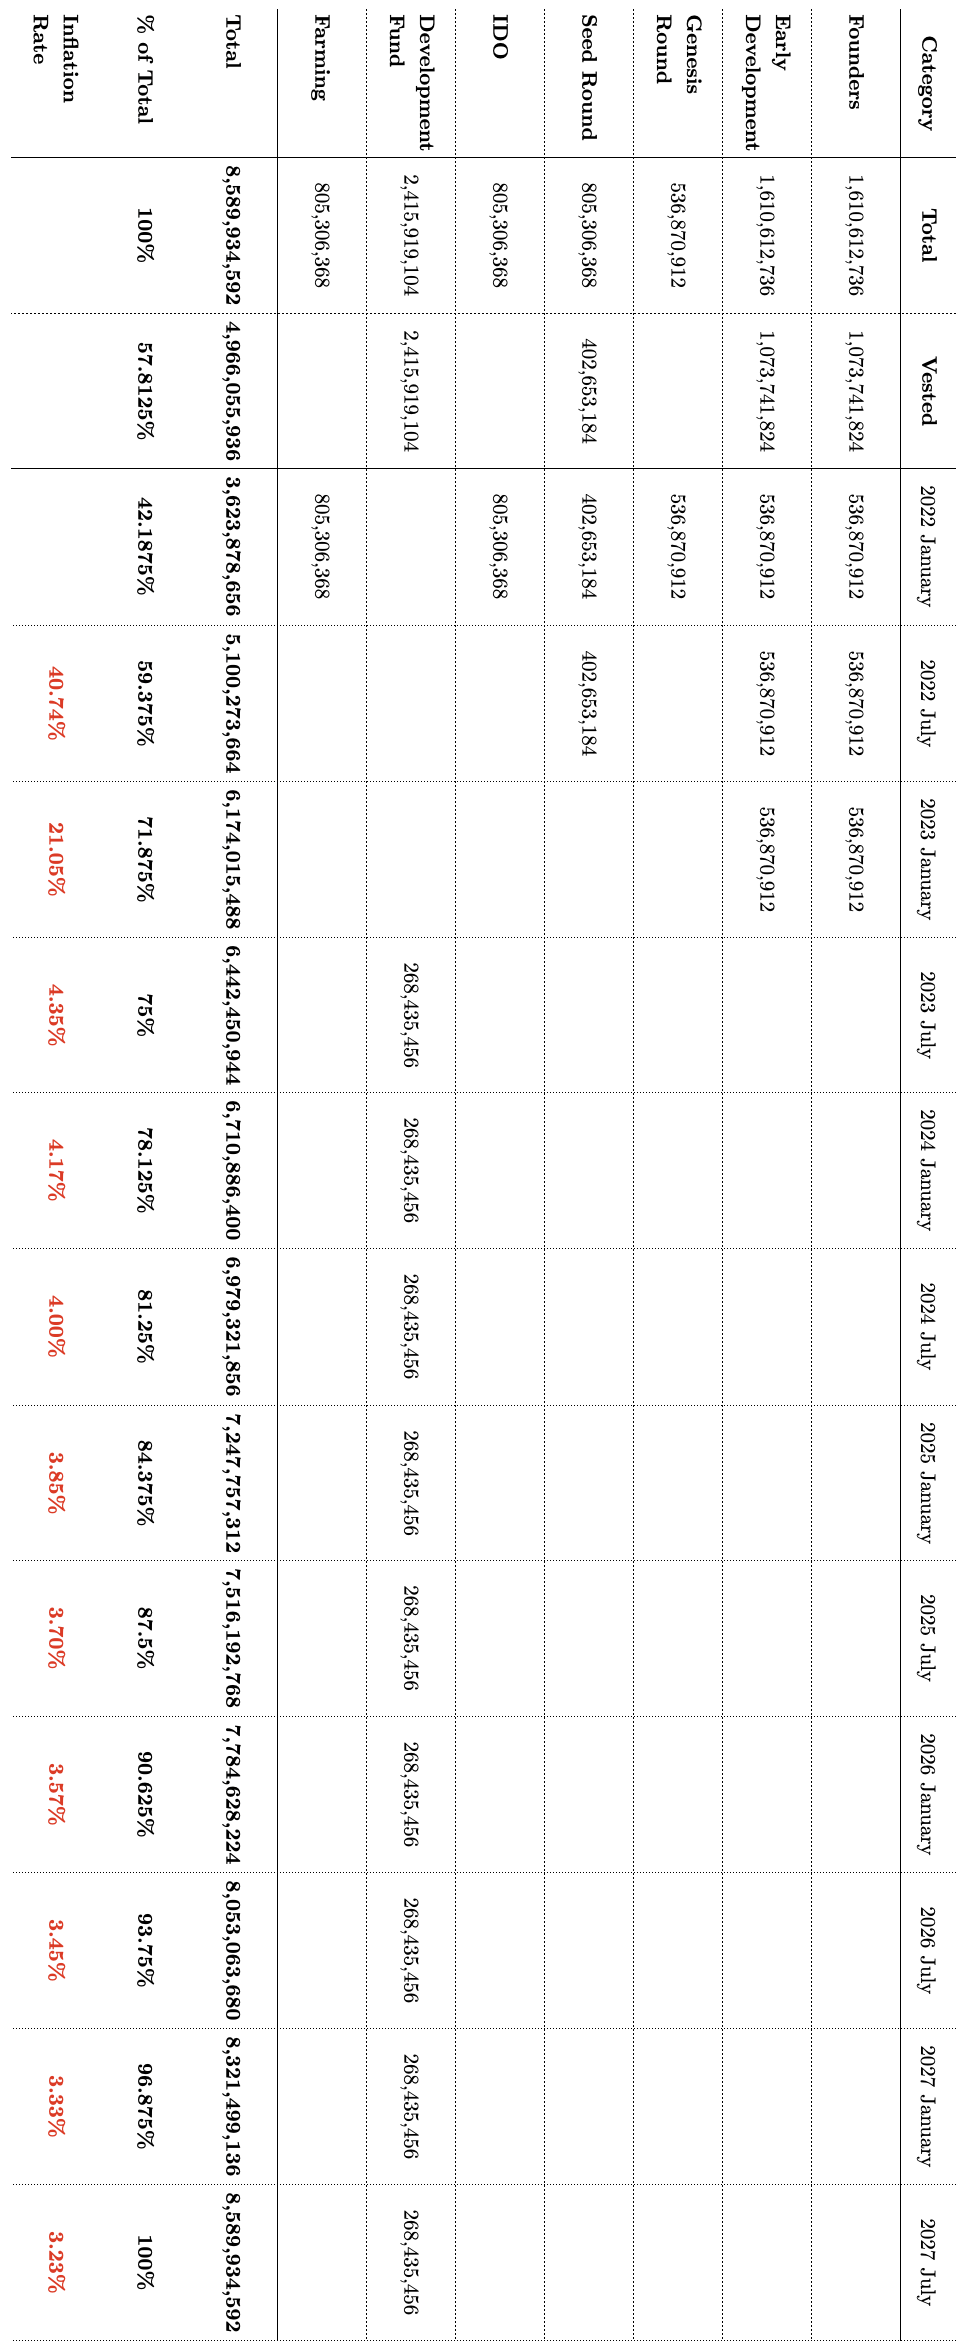
\includegraphics[width=3.5in]{images/The_Unit_Allocation_Table_2.png}
  \caption{Allocation details showing inflation rate.}
  \label{fig:allocation_table2}
\end{figure}






\section{Development Roadmap}

The Unit's ideas started in 2018; however, it was not as necessary in the crypto space then as it is today. Therefore, the project began testing the hypothesis of an algorithmic unit of account in 2020, and in 2021 it is running strong towards executing the plan.

We first launched The Unit algorithm online on May 5, 2021 (5/5/5). Currently, we are working on two-week blocks improving the functionality and all aspects of the product.

We are preparing a Uniswap proposal to include The Unit as a unit of account in their prices. Through this proposal, we intend to attract other defi projects to adopt The Unit.


\begin{thebibliography}{[BLSWZ9]}
\bibliographystyle{amsalpha}

\bibitem[B1]{B1} Basabe, I.: The Unit: Establishing a Crypto-Native Unit of Account. \emph{https://github.com/toknowwhy/the-unit-paper} (2020).


\bibitem[B2]{B2} Basabe, I.: 2ØY's (To Know Why) Values. \emph{https://github.com/toknowwhy/20y-values-paper} (2019).



\end{thebibliography}



\end{document}
